% /Users/claudio/overleaf/paper-section-warping/scripts/rectangle.py
{
\newcommand{\tw}{t_w}

\newcommand{\YieldStress}{Y}
\newcommand{\Hiso}{H_{\mathrm{iso}}}
\newcommand{\Hkin}{H}
\newcommand{\KinRate}{b}
\newcommand{\IsoRate}{\delta}
\newcommand{\BackStress}{\boldsymbol{x}}
\newcommand{\FlowStress}{Y}
\newcommand{\PlasticStrain}{\bm{E}^{\rm p}}
\newcommand{\RelativeStress}{\bm{\xi}} %{\bar{\bm{\sigma}}}
\newcommand{\PartialStress}{\bm{a}}
\newcommand{\StressNormal}{\bm{n}}
\newcommand{\EpPlEq}{\bar{\varepsilon}_{\rm p}}
\newcommand{\MisesStrain}{{\bar{\varepsilon}_{\rm p}}}
\newcommand{\NormScale}{\phi(\FlowUnit)}
\newcommand{\BackScale}{c_{\varphi}}
\newcommand{\MisesScale}{j_2}
\newcommand{\FlowRate}{\beta_\varepsilon}
\newcommand{\NormRate}{\beta_L}

% \begin{Quote}\textbf{Notes:}
% Compare with section 5.3.2 of \cite{saritas2006mixed}. \cref{fig:A} is a temporary placeholder taken from Di Re. I will draw a new one, and the units will of course, be Roman.
% \end{Quote}

\begin{figure}[H]
  \centering

  \begin{subfigure}[c]{0.55\linewidth}
    \centering
    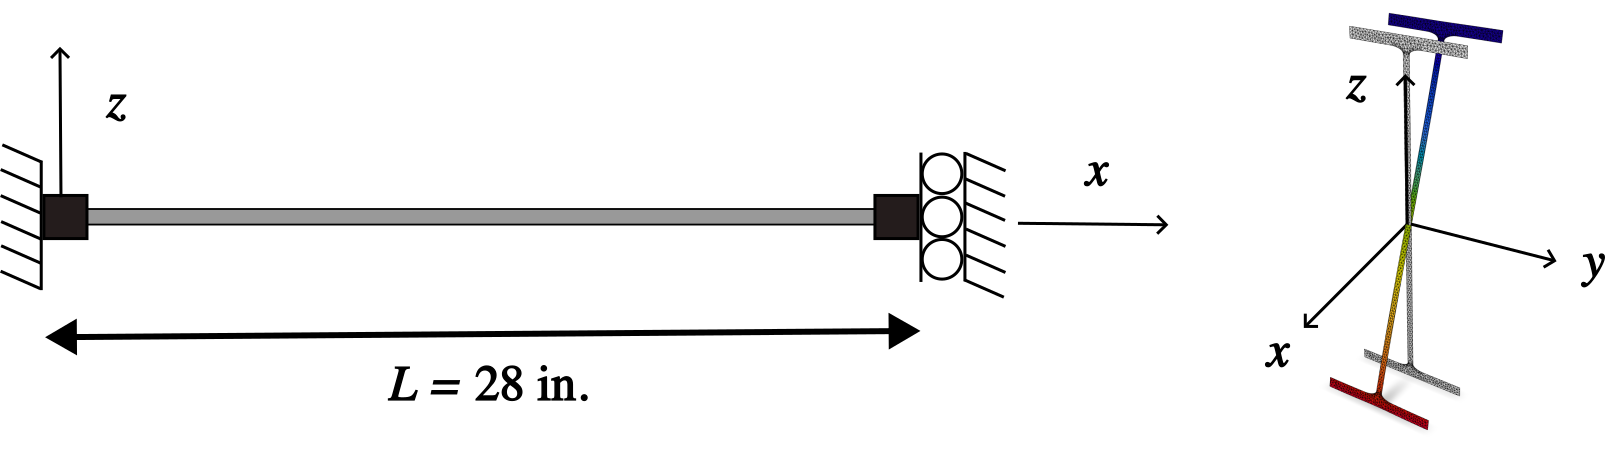
\includegraphics[width=\linewidth]{Figures/frame-2007.png}
    \caption{Finite element model.}
    \label{fig:2007-A}
  \end{subfigure}
  % \hfill
  \begin{subfigure}[c]{0.4\linewidth}
    \centering
    % 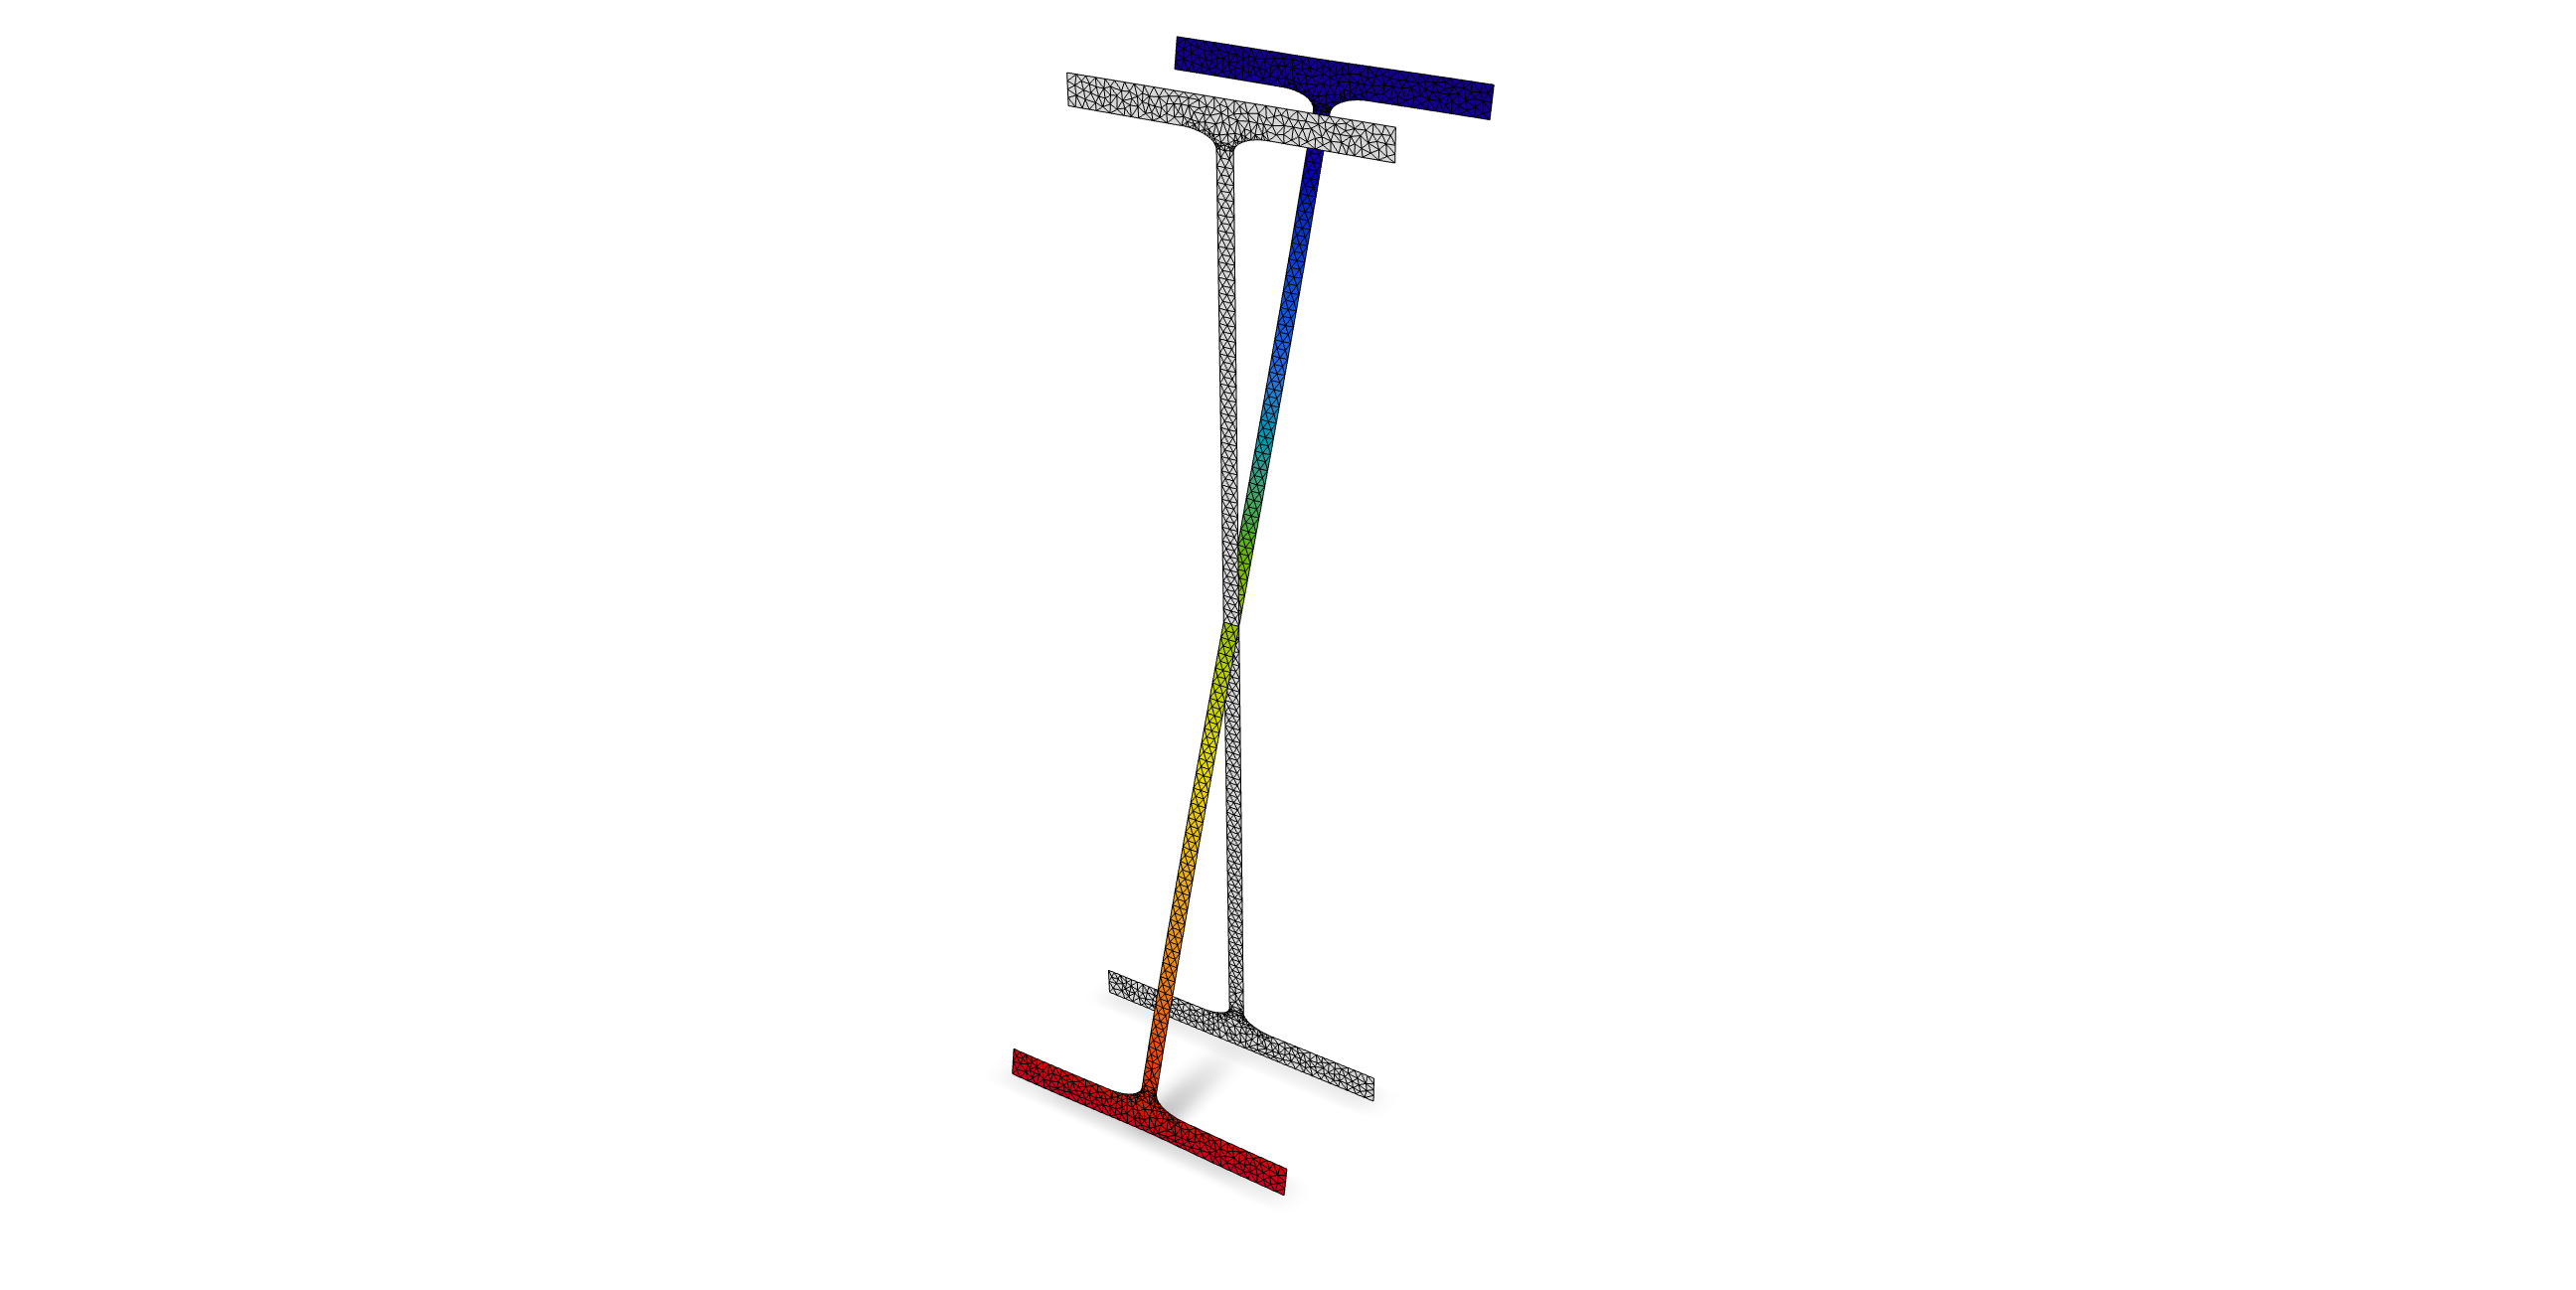
\includegraphics[width=\linewidth,trim={12cm 0 12cm 0},clip]{Figures/w18x40-warp.png}
    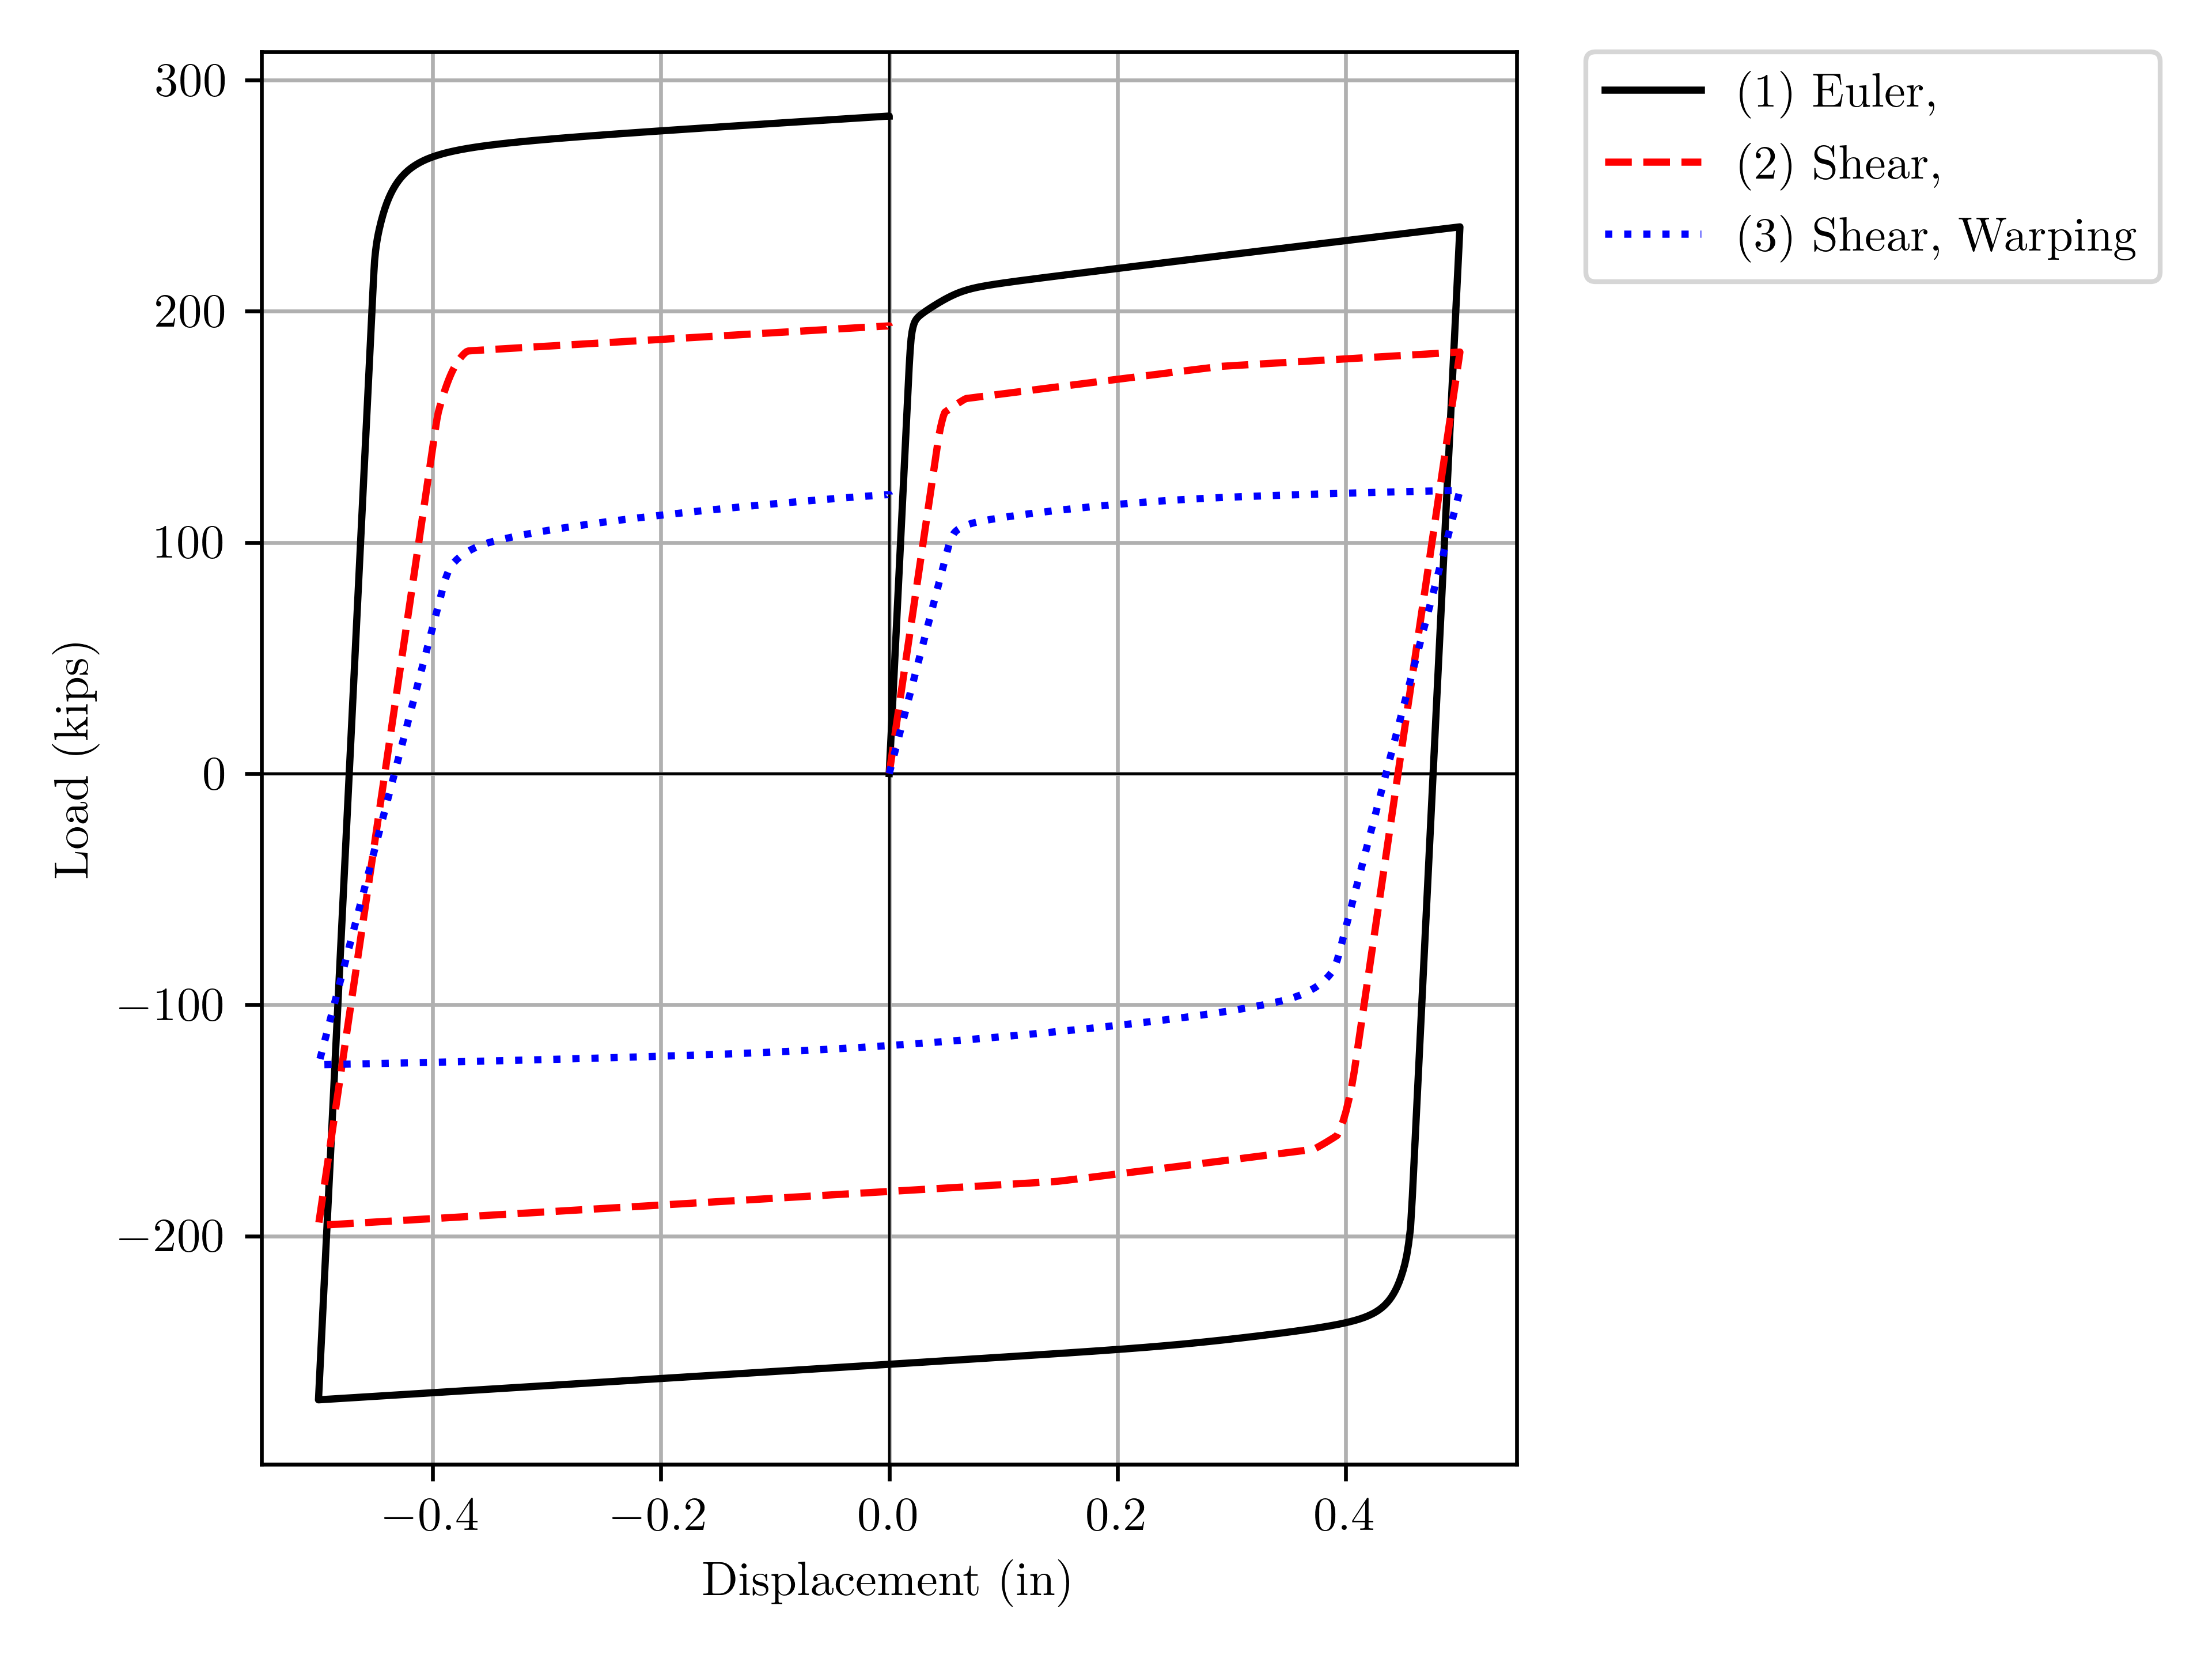
\includegraphics[width=\linewidth]{Figures/shear-link-response.png}
    \caption{Shear force \(V_y\) vs. displacement \(u_y\) at \(\reflenx=L\).}
    \label{fig:2007-C}
  \end{subfigure}
  
    \caption{Model of the steel shear link from Example~\ref{sec:frame-2021}.}
    \label{fig:shear-link}
\end{figure}

The built-in span in \cref{fig:2007-A} represents a shear link with a steel W18x40 section. 
Three formulations are considered: (1) a standard shear-free force formulation \citep{taucer1991fiber}, (2) the shear-deformable formulation of \cite{taylor2003mixed} with a section that neglects cross sectional warping (i.e., \(\WarpShearIesan_y =0\)), and (3) the same shear-deformable force formulation with a section that includes the warping mode \(\WarpShearIesan_y\) in \cref{fig:2007-A}. 
%
All cases use the multiaxial \(J_2\) plasticity model with yield stress \(f_y = 35\) ksi, and linear isotropic and kinematic hardening with moduli \(H_{\rm iso} = H_{\rm kin} = 0.002E\). 
The shear correction factor for this section is \(A/A_y = 0.46\) according to \cite{cowper1966shear}. 
For the analysis a displacement cycle is imposed at the end \(\reflenx=L\). 
The enriched section matches the elastic stiffness exactly. 
\begin{figure}[H]
    \centering
    \begin{subfigure}[c]{0.5\linewidth}
    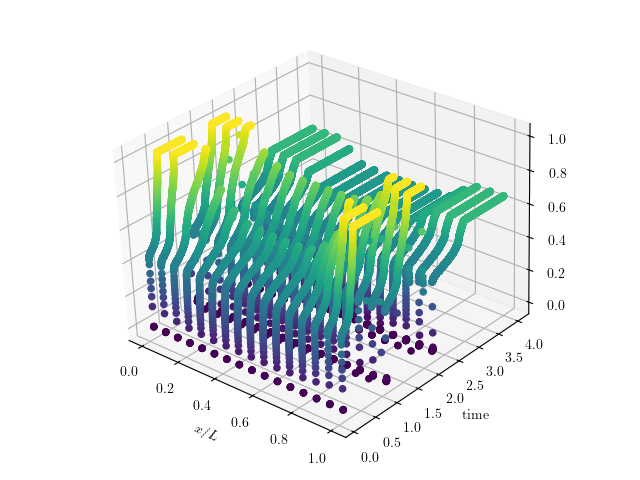
\includegraphics[width=0.9\linewidth]{Examples//frame-2007/2007-plastic-spread.png}
    \caption{Plastic spread over time.}
    \end{subfigure}
    \begin{subfigure}[c]{0.3\linewidth}
        
    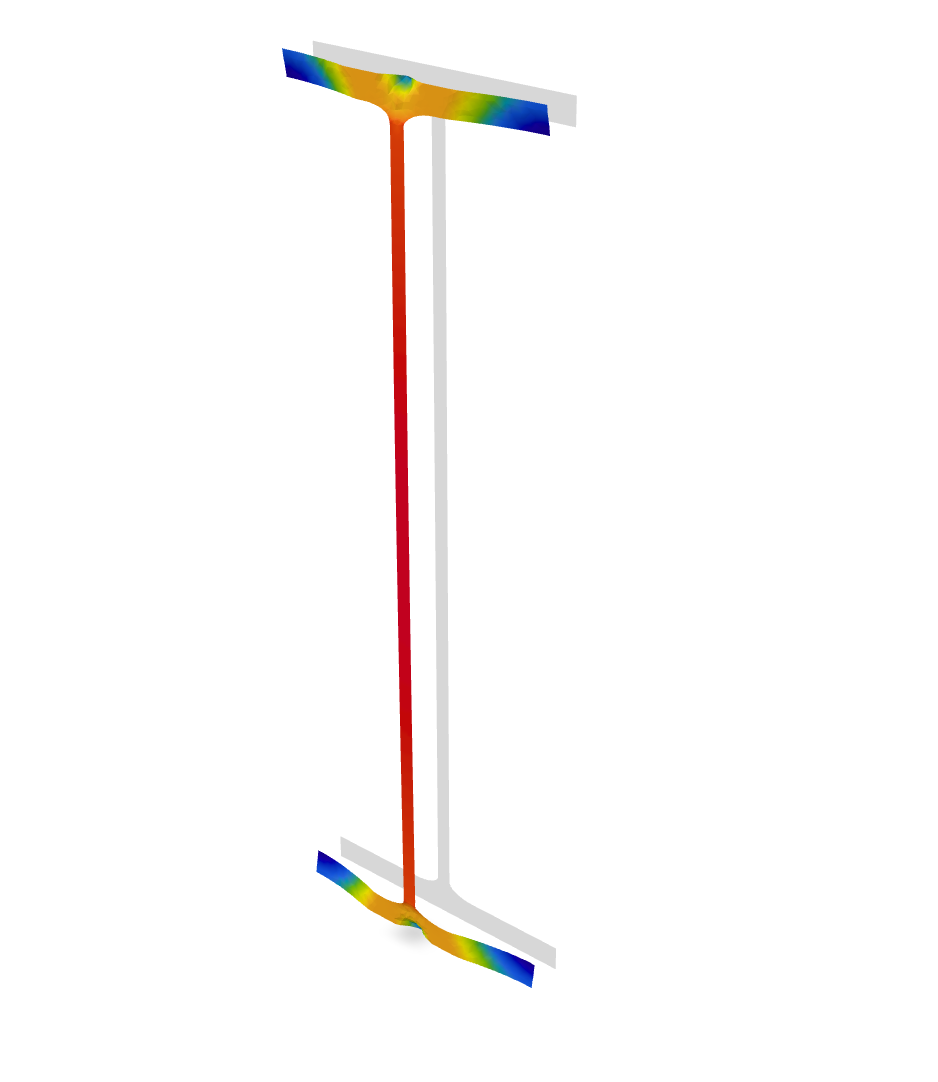
\includegraphics[width=0.9\linewidth]{Examples//frame-2007/2007-section-1.png}
    \caption{$J_2$ stress in section 1 at the end of the simulation.}
    \end{subfigure}
\end{figure}

\cref{fig:2007-C} reports the transverse \((y)\) shear force -- displacement response at the point of imposed displacement \(\reflenx=L\). The significant impact of shear and warping deformations is evident. 
A section that incorporates shear deformations without warping fails to reproduce the elastic stiffness and overestimates both the strength and the energy dissipation.

}

\FrameSection{
label/problem=frame-2007,
label/shape={W18x40},
% Section
shape={Wide Flange},
kinematics/section={\eqref{eq:linear-gl-strain-pi}},
unit/length={\inch}
}